\documentclass{beamer}

\usepackage[polish]{babel}
\usepackage[T1]{fontenc}
\usepackage[utf8]{inputenc}
\usepackage{txfonts}
\usepackage{amsmath}
\usepackage{algorithm2e}

\usetheme{Warsaw}

\title{Problem dystrybucji towarów z najwcześniejszymi i najpóźniejszymi terminami dostaw} 
\author{Dawid Ryznar, Krzysztof Zielonka}

\date{5 Grudnia 2012}

\begin{document}

\frame{\titlepage}

\begin{frame}
	\begin{block}{Opis problemu (orginalny)}
		Jako firma transportowa mamy dostarczyć towary do miast. 
		Każde miasto ma ustaloną kare za spóźnienie lub przybycie zawcześnie. 
		Przemieszczenia się między miastami trwa pewną liczbę czasu.
		Należy znalęść ciąg miast, dla którego ciężarówka odwiedza każde miasto i minimalizujący sumę kar jaką trzeba zapłacić za zbyt wczesne lub zbyt późne przybycie.
		%\begin{itemize}
		%	\item Należy dostarczyć towary do miast
		%	\item Każde miasto ma określone terminy, w których należy dostarczyć towar
		%	\item Przemieszczanie miedzy miastami zajmuje pewien czas
		%	\item Nidotrzymanie terminu wiąże się z otrzymaniem kary
		%	\item Rozwiązaniem problemu jest ciąg miast, który minimalizuje koszt dostarczenia towarów do wszystkich miast.
		%\end{itemize}
	\end{block}
\end{frame}

\begin{frame}
	\begin{block}{Nasze założenia}
		\begin{itemize}
			\item Ciężarówka ma nieskończoną pojemność (jest w stanie zabrać towary dla wszystkich miast).
			\item Dla każdego miasta mamy funkcje kary od czasu (ogólniejszy wariant kar).
			\item Czas jest w postaci liczby naturalnej (np liczba sekund).
			\item Znamy pewne górne ogranicznie czasowe, które okresla maksymalny czas przejazdu.
			\item Rozładunek i załadunek nie wymaga czasu.
			\item W kązdym miesic możemy czekać dowolną liczbe czasu znim wyładujemy towar.
			\item Znamy wierzchołek startowy (magazyn).
		\end{itemize}
	\end{block}
\end{frame}

\begin{frame}
	\begin{block}{Instancja problemu}
		Miastom przyporządkowujmey numery.
		Instancją problemu jest para:
		\begin{equation}
			P = \left< T, p \right>
		\end{equation}
	\end{block}
	\begin{block}{Macierz czasu przajazdów}		
		\begin{equation}
			T = \left[ t_{ij} \right]_{n \times n} 
		\end{equation}
		Kwadratowa maciarz gdzie element $t_{ij}$ to czas potrzebny na przejazd najszybszą drogą z miasta $i$ do $j$.
	\end{block}
	\begin{block}{Funkcja kary}
		\begin{equation}
			p : N \rightarrow N \rightarrow R 
		\end{equation}
		Funkcja kary, przyjmująca kolejno numer miasta, czas rozładunku i zwracająca karę w postaci liczby rzeczywistej.
	\end{block}
\end{frame}



\begin{block}{Opis problemu}
\begin{itemize}
	\item Pełny graf ważony z $n$ wierzchołkami,
	\item Wyróżniony jeden wierzchołek startowy $v_{start}$
	\item Wprowadzmy funckje kary $p$ jaką trzeba zapłacić za dostarczenie towaru w czasie $t$ do pewnego miasta (bardziej ogólny wariant, miasta mogą nadawać kary bardziej swobodnie oraz mogą nadawać nagorody)
	\item Każda krawędź ma przyparzadkowany czas potrzebny na jej pokonanie.
	\item Dodatkowo zakładamy, że w każdym mieście możemy przeczekać pewien okres czasu.
	\item Dla uproszczenie zakładamy, że jest pewne górne ograniczenie na czas potrzebny na pokonaniem trasy. Jeżeli rozwiązanie potrzebuje więcej czasu zakładamy, że jest ono nieakceptowalne.
\end{itemize}
\end{block}


\begin{frame}{Opis problemu}
	
	\begin{equation}
		DT = \left< V, w, p, t_{max}\right>
	\end{equation}
	\begin{equation}
		t : V \rightarrow N
	\end{equation}
	\begin{equation}
		p : V \times N \rightarrow R
	\end{equation}
	\begin{description}
		\item[$w$] -- przyporządkowuje krawędziom wagi (czasy podróży)
		\item[$p$] -- funckja kary, dla danego wierzchołka i czasu przybcia zwraca kare w postaci liczby rzeczywistej
		\item[$t_{max}$] -- górne ograniczenie na czas potrzebny na pokonaniem dystansu
	\end{description}

\end{frame}

\begin{frame}
	
	\begin{block}{Instancja problemu}
		Miastom przyporządkowujmey kolejno numery $2, \cdots, n$.
		Dla uproszczenia będziemy zakładać, że magazyn zawsze ma numer $1$.
		Instancją problemu jest para:
		\begin{equation}
			P = \left< T, p \right>
		\end{equation}
	\end{block}
	
	\begin{block}{Macierz czasu przajazdów}		
		\begin{equation}
			T = \left[ t_{ij} \right]_{n \times n} 
		\end{equation}
		Kwadratowa maciarz gdzie element $t_{ij}$ to czas potrzebny na przejazd najszybszą drogą z miasta $i$ do $j$.
	\end{block}
	
	\begin{block}{Funkcja kary}
		\begin{equation}
			p : N \rightarrow N \rightarrow R 
		\end{equation}
		Funkcja kary, przyjmująca kolejno numer miasta, czas rozładunku i zwracająca karę w postaci liczby rzeczywistej.
	\end{block}

\end{frame}

\begin{frame}{Graf miast}
		
	W grafie miast, wierzchołki interpretujemy jako miasta, a wagi na krawędziach jako czasy potrzebne na przedostanie sie z jednego miasta do drugiego.
	Czas na krawędzi $\{u, v\}$ jest najszybszym czasem potrzebnym na przedostanie sie z miasta $u$ do $v$.
	\begin{itemize}
		\item Graf miast spełnia nierówność trójkąta
			\begin{equation}
				a < b + c \ \wedge \ b < a + c \ \wedge \ c < a + b
			\end{equation}
			\begin{equation}
				\forall_{a,b,c \in V} t(\left\{a, c\right\}) < t(\left\{a, b\right\}) + t(\left\{b, c\right\})
			\end{equation}
		\item Graf miast jest grafem pełnym
	\end{itemize}
	Jeżeli graf niespłnia jednego z powyższych założen to możemy go do takiego przekonwertować wywołujac dla każdego wierzchołka $BFS$.

\end{frame}


\begin{frame}{Nierówność trójkąta}
	
	\begin{equation}
		a < b + c \ \wedge \ b < a + c \ \wedge \ c < a + b
	\end{equation}
	\begin{itemize}
		\item Zakładamy, że dany czas przejazdu między dowolnymi dwoma miastami to średni czas potrzebny na pokonanie najszybszej trasy łączącej te dwa miasta
		\item Dzięki temu założeniu graf dla miast spełnia nierówność trójkąta czyli:
			\begin{equation}
				\forall_{a,b,c \in V} t(\left\{a, c\right\}) < t(\left\{a, b\right\}) + t(\left\{b, c\right\})
			\end{equation}
		\item Eleminujemy możliwość rozwiązania gdzie miasta mogą sie powtarzać, jeżeli mamy dostarczyć towar do miasta $b$, a znajdujemy sie w mieścia $a$ to najszybsza droga między tymi miastami zajmuje $t(\left\{a, b\right\})$
	\end{itemize}

\end{frame}


\begin{frame}
	
	\begin{block}{Rozwiązania dopuszczalne}
		Rozwiązaniem dopuszczalnym (sepłniającym warunki zadania) jest permutacja liczb $1, \cdots, n$.
	\end{block}

	\begin{block}{Uzasadnienie}
		\begin{itemize}
			\item W rozwiązniu musza znaleść sie wszystkie miasta. (definicja problemu)
			\item W rozwiązaniu miasta nie mogą sie powtarzać. (nierówność trójkąta
				+ założenie o nieskończonej ładowności ciężarówki
				+ możliwość czekania w dowolnym mieście)
			\item W rozwiazniu nie uwzgledniamy magazynu. (to jest punkt startowy i końcowy
				+ założenie o nieskończonej ładowności ciężarówki)	
		\end{itemize}
	\end{block}

\end{frame}

\begin{frame}{Funkcja celu}
		
		\begin{equation}
			F : N^n \rightarrow R
		\end{equation}
		\begin{equation}
			F(v_1 \cdots v_n) = C(v_1, \cdots V_n, 0)
		\end{equation}

\end{frame}

\begin{frame}{Funkcja pomocnicza}
		
		\begin{equation}
			C : N^m \times N \rightarrow R \ \ \ \text{gdzie} \ m > 0
		\end{equation}
		\begin{equation}
			C(v, t) = \begin{cases}
				p(v, t)	&	\text{gdy} \ t < t_{max} 	\\
				+inf	&	\text{wpp}			\\
			\end{cases}
		\end{equation}
		\begin{equation}
			C(v_1, \cdots, v_n, t) = \min\limits_{t \leq t_c \le t_{max}}\left\{ C(v_2, \cdots, v_n, t_c + t_{1,2}) + p(v_1, t_c) \right\}
		\end{equation}

\end{frame}

\begin{frame}{Złożonośc problemu}
	\begin{block}{Złożnosc problemu}
		Problem dystrupucji towarów jest NP trudny.
		Udowodnimy to konstrująć wielomianową redukcje problemu komiwojażera do problemu dystrybucji towarów.
	\end{block}

	\begin{block}{Problem komiwojażera}
		Mamy dany pełny ważony graf G. Rozwiązaniem problemu jest minimalny cykl Hamiltona na tym grafie.
	\end{block}
\end{frame}

\begin{frame}{Złożonośc problemu}
	\begin{block}{Dowód}
		
		\begin{algorithm}[H]
			\KwData{G -graf pełny wazony, w - funkcja wagowa}
			\KwResult{trojka $\left<T, p, t_{max}\right>$}
			$f$ -- funkcja przyporządkowywujaca wierzchołkom grafu kolejne liczby naturalne \\
			$g$ -- funkcja przyporządkowwywująca krawędziom kolejne liczby naturalne \\
			$p(v, t) = \lambda\left( v, t \right) \rightarrow \sum_{\{u, v\} \in E} (2^{g(\left\{u, v\right\})} \& t) \cdot w(\left\{ u, v \right\}) $ \\
			\ForAll{$v, u \in V$}{
				$T[f(v), f(u)] = 2^{g(\left\{v,u\right\})}$ \\
			}
			$t_{max} = \sum\limits_{i=2}^{|V|} w(f(v_{i-1}), f(v_i))$ \\
			\Return $\left< T, p , t_{max} \right> $
		\end{algorithm}
	
	\end{block}

\end{frame}


\begin{frame}{Algorytm konstrukcyjny}
	
	\begin{block}{Opis algorytmu konstrukcyjnego}
		Algorytm konstrukcyjny oparliśmy na podstawie algorytmu Local Search. 
		Ssąsiądów wybieramy wykorzystując wszystkie możliwe transpozycje.
		
	\end{block}

	\begin{block}{Local Search}
		\begin{algorithm}[H]
			\KwData{$x$ -- initial node}
			
			\KwResult{$best\_neighbour$ -- the best local node}
			$current = none$ \\
			$best\_neighbor = x$ \\
			\Repeat{$F(best_neighbour) = = F(current)$}{
				$current = best\_neighbour$
				$neighbours = $ find all neighbours of $current$
				$best\_neighbour = $ select best from $neighbours \cup \left\{current\right\}$				
			}
			\Return $best\_neighbour$
		\end{algorithm}
	\end{block}

\end{frame}

\begin{frame}{Algorytm konstrukcyjny}

	\begin{block}{Neighbors}
		\begin{algorithm}[H]
			\KwData{x -- current node}
			\KwResult{neighbours -- set of x's neighbours}
			$ neighbours = \empty $ \\
			\ForAll{$1 \leq i, j \leq n \ \wedge i < j$}{
				$neighbours \cup= x_1 \cdots x_{i-1}, x_j, x_{i+1} \cdots x_{j-1}, x_i, x_{j+1} \cdots x_n$
			}
			\Return neighbours
		\end{algorithm}
	\end{block}

\end{frame}

\begin{frame}{Algorytm konstrukcyjny}

	\begin{block}{Algorytm konstrykcyjny dla problemu dystrybucji towarów}

		\begin{algorithm}[H]
			\KwData{$T, p, t_{max}, x$ -- initial node}
			\KwResult{$best\_neighbor$ -- best local neighbour}
			$ current = none $ \\
			$ best\_neighbor = x $ \\
			\Repeat{$F(best_neighbour) = = F(current)$}{
				$current = best\_neighbor$
				$neighbours = Neighbours(x) \cup \left\{current\right\}$
				$best\_neighbour =  $ select best from $neighbours$
			}
			\Return $best\_neighbor$
		\end{algorithm}
	\end{block}

\end{frame}


\begin{frame}{Symulowane wyżarzanie [ang. \textit{Simulated Annealing}]}

	\begin{block}{}
	Rodzaj algorytmu heurystycznego przeszukującego przestrzeń alternatywnych rozwiązań problemu w celu wyszukiwania rozwiązań najlepszych. Jest wariantem metody przeszukiwania lokalnego [ang. \textit{Local Search}].
	Ogólny szkic działania algorytmu symulowanego wyżarzania:
	\end{block}
	\begin{enumerate}
		\item losowy wybór punktu startowego
		\item losowy wybór sąsiada
		\item odpowiednia akceptacja sąsiada
		\item po każdej iteracji temperatura zostaje zaktualizowana:
			$$ T = n\cdot T \wedge n \in (0,1)$$
		\item algorytm zatrzymuje się gdy w ciągu ustalonej liczby iteracji nie uda się osiągnąć lepszego wyniku
	\end{enumerate}

\end{frame}

\begin{frame}{Symulowane wyżarzanie [ang. \textit{Simulated Annealing}]}

    \begin{algorithmic}[H]
    \State $n -- \ \text{dlugosc permutacji}$
    \While{$k = 0 to n^3$}{
    }
    \end{algorithmic}
	\scalebox{0.4}{
	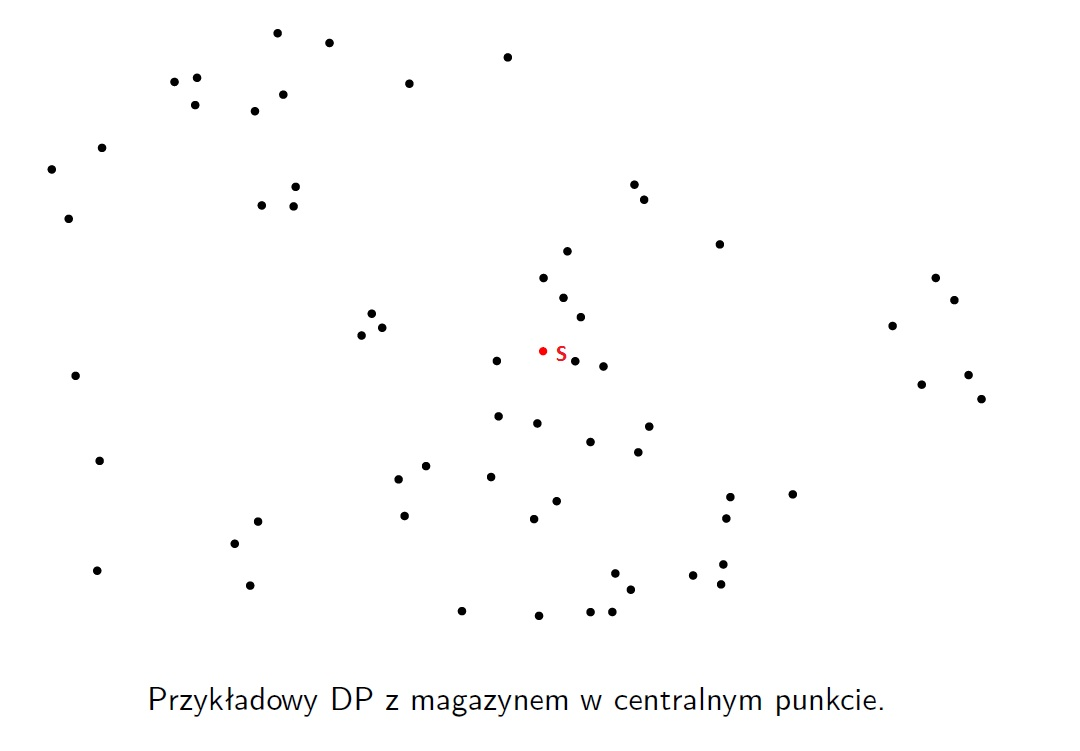
\includegraphics{./slajdy/1.jpg}}

\end{frame}

\begin{frame}{Symulowane wyżarzanie [ang. \textit{Simulated Annealing}]}

	\scalebox{0.4}{
	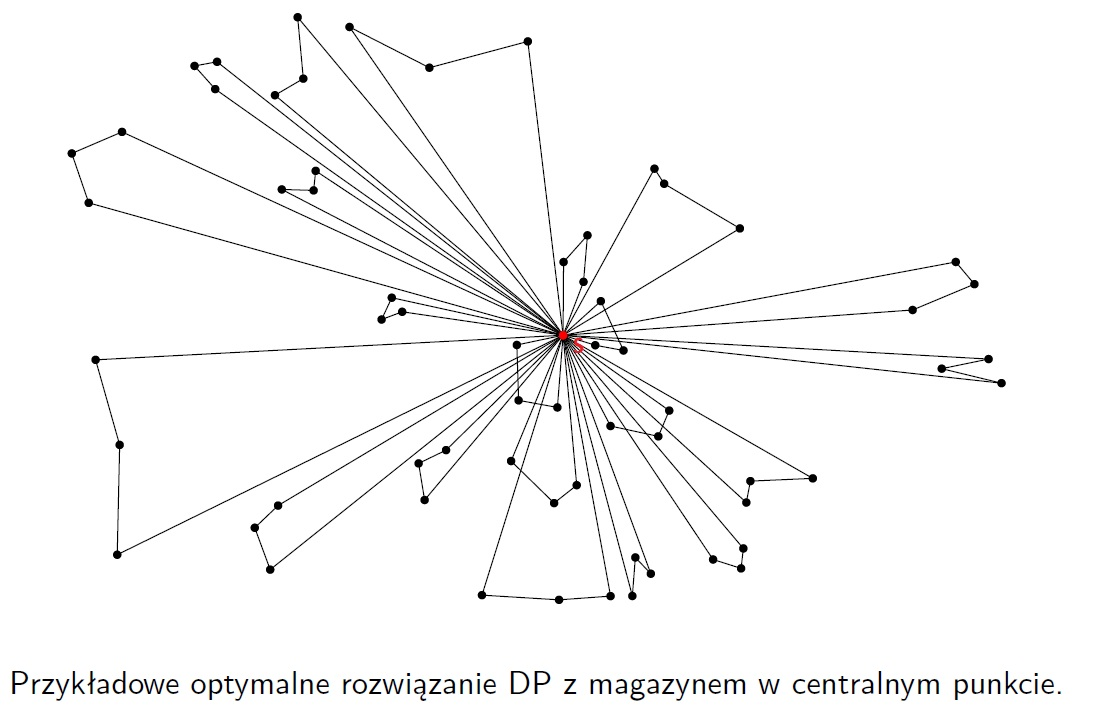
\includegraphics{./slajdy/2.jpg}}

\end{frame}

\begin{frame}{Symulowane wyżarzanie [ang. \textit{Simulated Annealing}]}
	
	\scalebox{0.4}{
	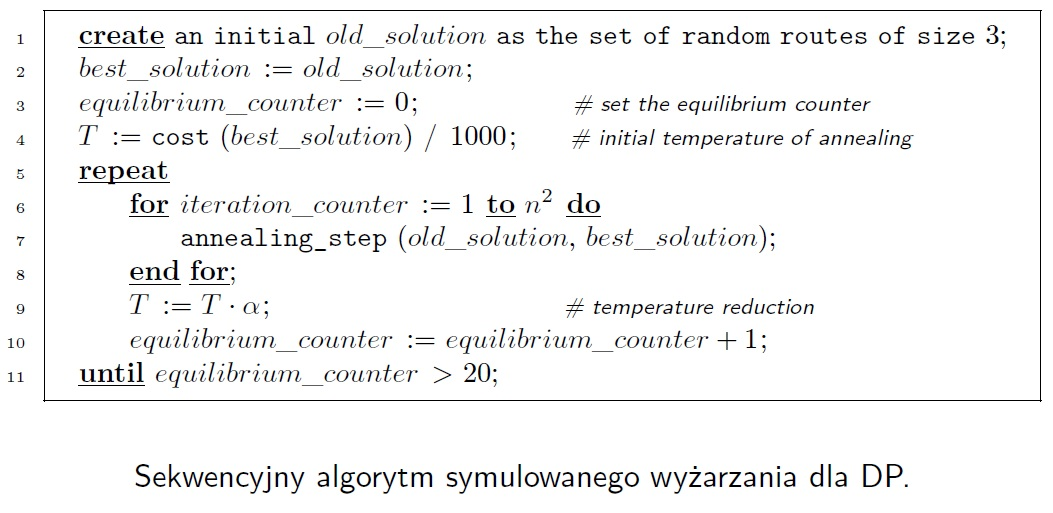
\includegraphics{./slajdy/3.jpg}}

\end{frame}

\begin{frame}{Symulowane wyżarzanie [ang. \textit{Simulated Annealing}]}

	\scalebox{0.4}{
	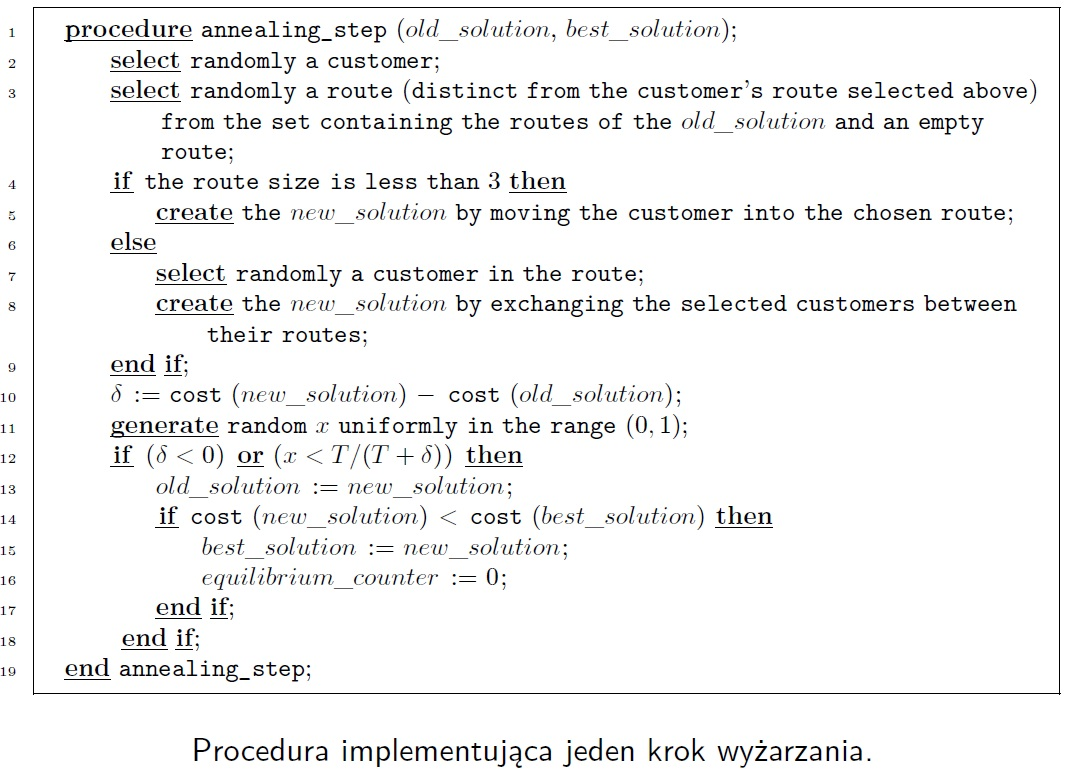
\includegraphics{./slajdy/4.jpg}}

\end{frame}


\begin{frame}{Wykonanie}

	\begin{block}{}
	Projekt wykonano przy użyciu:
	\end{block}
	\begin{enumerate}
		\item Ruby (język programowania)
		\item Git (CVS)
		\item RubyMine (IDE)
	\end{enumerate}
	\begin{block}{}
	Projekt ma swoje repozytorium w serwisie github.com
	
	\url{https://github.com/kzielonka/Praktyka-Optymalizacji-Projekt}
	\end{block}
	

\end{frame}


\end{document}